\documentclass[11pt,a4paper]{article}

\usepackage[margin=2.2cm]{geometry}
\usepackage[T1]{fontenc}
\usepackage{lmodern}
\usepackage{microtype}
\usepackage{amsmath}
\usepackage{graphicx}
\usepackage{booktabs}
\usepackage{tabularx}
\usepackage{array}
\usepackage{xcolor}
\usepackage{enumitem}
\usepackage{listings}
\usepackage{fancyhdr}
\usepackage{caption}
\usepackage{float}
\usepackage{longtable}
\usepackage[hidelinks]{hyperref}

\newcommand{\TeamName}{The CodeSmiths}
\newcommand{\MemberOne}{Srivathsav}
\newcommand{\RegOne}{106125061}
\newcommand{\MemberTwo}{Manmeet}
\newcommand{\RegTwo}{106125063}
\newcommand{\MemberThree}{Manthan}
\newcommand{\RegThree}{106125065}

\definecolor{codebg}{HTML}{F6F8FA}
\definecolor{codekw}{HTML}{1F4E79}
\definecolor{codecm}{HTML}{5B7B5B}
\lstset{
  language=C++,
  basicstyle=\ttfamily\footnotesize,
  keywordstyle=\color{codekw}\bfseries,
  commentstyle=\color{codecm}\itshape,
  backgroundcolor=\color{codebg},
  frame=single,
  rulecolor=\color{black!25},
  breaklines=true,
  tabsize=4,
  showstringspaces=false,
  xleftmargin=2pt,
  xrightmargin=2pt,
  aboveskip=6pt,
  belowskip=4pt
}

\setlist{itemsep=2pt, topsep=4pt}
\setlength{\parindent}{0pt}
\setlength{\parskip}{5pt}
\renewcommand{\arraystretch}{1.15}
\captionsetup{font=small, labelfont=bf}

\pagestyle{fancy}
\fancyhf{}
\fancyhead[L]{\small CampusFlow -- CSLR31 Data Structures Laboratory Project}
\fancyhead[R]{\small \TeamName}
\fancyfoot[C]{\small\thepage}
\renewcommand{\headrulewidth}{0.3pt}

\newcommand{\code}[1]{\texttt{#1}}

\begin{document}

% =================================================================
%  TITLE + STEP 1 : ABSTRACT
% =================================================================
\begin{center}
  {\Large\bfseries CampusFlow}\\[4pt]
  {\large Venue Seating, Check-in and Crowd Evacuation Planner\\
  built on five hand-written data structures}\\[10pt]
  \textbf{Team:} \TeamName\\[4pt]
  \begin{tabular}{ll}
    \MemberOne & \RegOne\\
    \MemberTwo & \RegTwo\\
    \MemberThree & \RegThree
  \end{tabular}\\[6pt]
  CSLR31 -- Data Structures Laboratory Project Report
\end{center}

\section*{Step 1: Abstract}

\textbf{Problem and motivation.}
Campus events such as seminars, examinations and cultural programmes can bring
hundreds of people into a venue. When seating is managed manually, it becomes
hard to keep track of available seats, accommodate late arrivals fairly and
know how many people are present in each part of the hall. Seats may also remain
empty when registered participants do not show up. In an emergency, a blocked
exit or a crowded corridor can make it difficult to guide people along a safe
alternative route.

\textbf{Existing products.}
Online ticketing platforms allow users to choose seats, while crowd-monitoring
systems use cameras or sensors to estimate how many people are present. These
solutions usually handle separate parts of the problem and may require paid
services or additional hardware. CampusFlow brings seating, waiting-list
management and evacuation routing together in a single terminal-based program.

\textbf{Objectives.}
We developed CampusFlow as a terminal-based system with four main goals. It
registers participants and tries to seat each person in their preferred zone;
maintains a priority-based waiting list and assigns released seats to waiting
participants; reports occupancy and crowding levels for each zone; and finds
routes through the venue while taking congestion into account, including during
evacuation.

\textbf{Salient features.}
The system uses a hash table for participant lookup in $O(1)$ average time and
a segment tree to calculate zone totals and locate the first free seat in
$O(\log N)$. A min-heap selects the next participant from the waiting list
based on priority and arrival time. For movement around the venue, the graph
module uses Dijkstra's algorithm, BFS and a multi-source evacuation search.
Congestion alerts use hysteresis: they switch on at 80\% occupancy and switch
off at 70\%, which helps prevent alerts from repeatedly turning on and off.

\textbf{Future scope.}
There is room to extend the project with a graphical interface, persistence for
the waiting list, live head-counts through QR or RFID check-in, and our own
implementations of the standard containers that are still used in a few modules.

\textbf{Social cause and SDG alignment.}
CampusFlow is related to UNESCO's Sustainable Development Goal 11
(\emph{Sustainable Cities and Communities}) because it aims to make shared
spaces, including campus halls, safer and easier to manage. It also connects
with Goal 4 (\emph{Quality Education}), as better-organised campus events can
help make educational activities more accessible to registered participants
~\cite{unesco-sdg}.

% =================================================================
%  STEP 2 : DESIGN
% =================================================================
\section{Step 2: Design of the Product}

\subsection{Idea}
For this project, we represent the venue as a $6\times 8$ grid containing
48 seats. The grid is divided into three horizontal zones, with 16 seats in
each zone. Every participant is assigned a priority (0--9) and selects a
preferred zone. We built the design around four main ideas:

\begin{enumerate}
  \item \textbf{Keep occupancy data consistent.} Whenever a seat changes
        state, the seat grid updates the segment tree as part of the same
        operation. Reports get their counts from the tree instead of maintaining
        separate counters, which helps avoid mismatched values.
  \item \textbf{Handle a full venue fairly.} When no seat is available,
        participants are added to a min-heap. The heap considers priority first
        and join time next, so the participant with the best waiting-list rank
        is selected first.
  \item \textbf{Reuse seats after no-shows.} A participant gets a 15-minute
        grace period to check in. If they do not arrive, the system releases the
        seat and offers it to the next eligible person on the waiting list.
  \item \textbf{Connect seating with movement.} Before a graph operation is
        carried out, the occupancy of the three zone halls is refreshed from
        the segment tree. This allows the routing and evacuation calculations
        to use the latest occupancy information.
\end{enumerate}

\subsection{Flow chart}
Figure~\ref{fig:flow} gives an overview of how the program runs. It starts by
initialising the data structures and then displays the main menu. After the
user selects an option, the corresponding operation is performed and control
returns to the menu. This continues until the user selects option 0 to exit.
We created the flow chart using Graphviz and included it in the report as
\code{flowchart.pdf}.

\begin{figure}[ht]
  \centering
  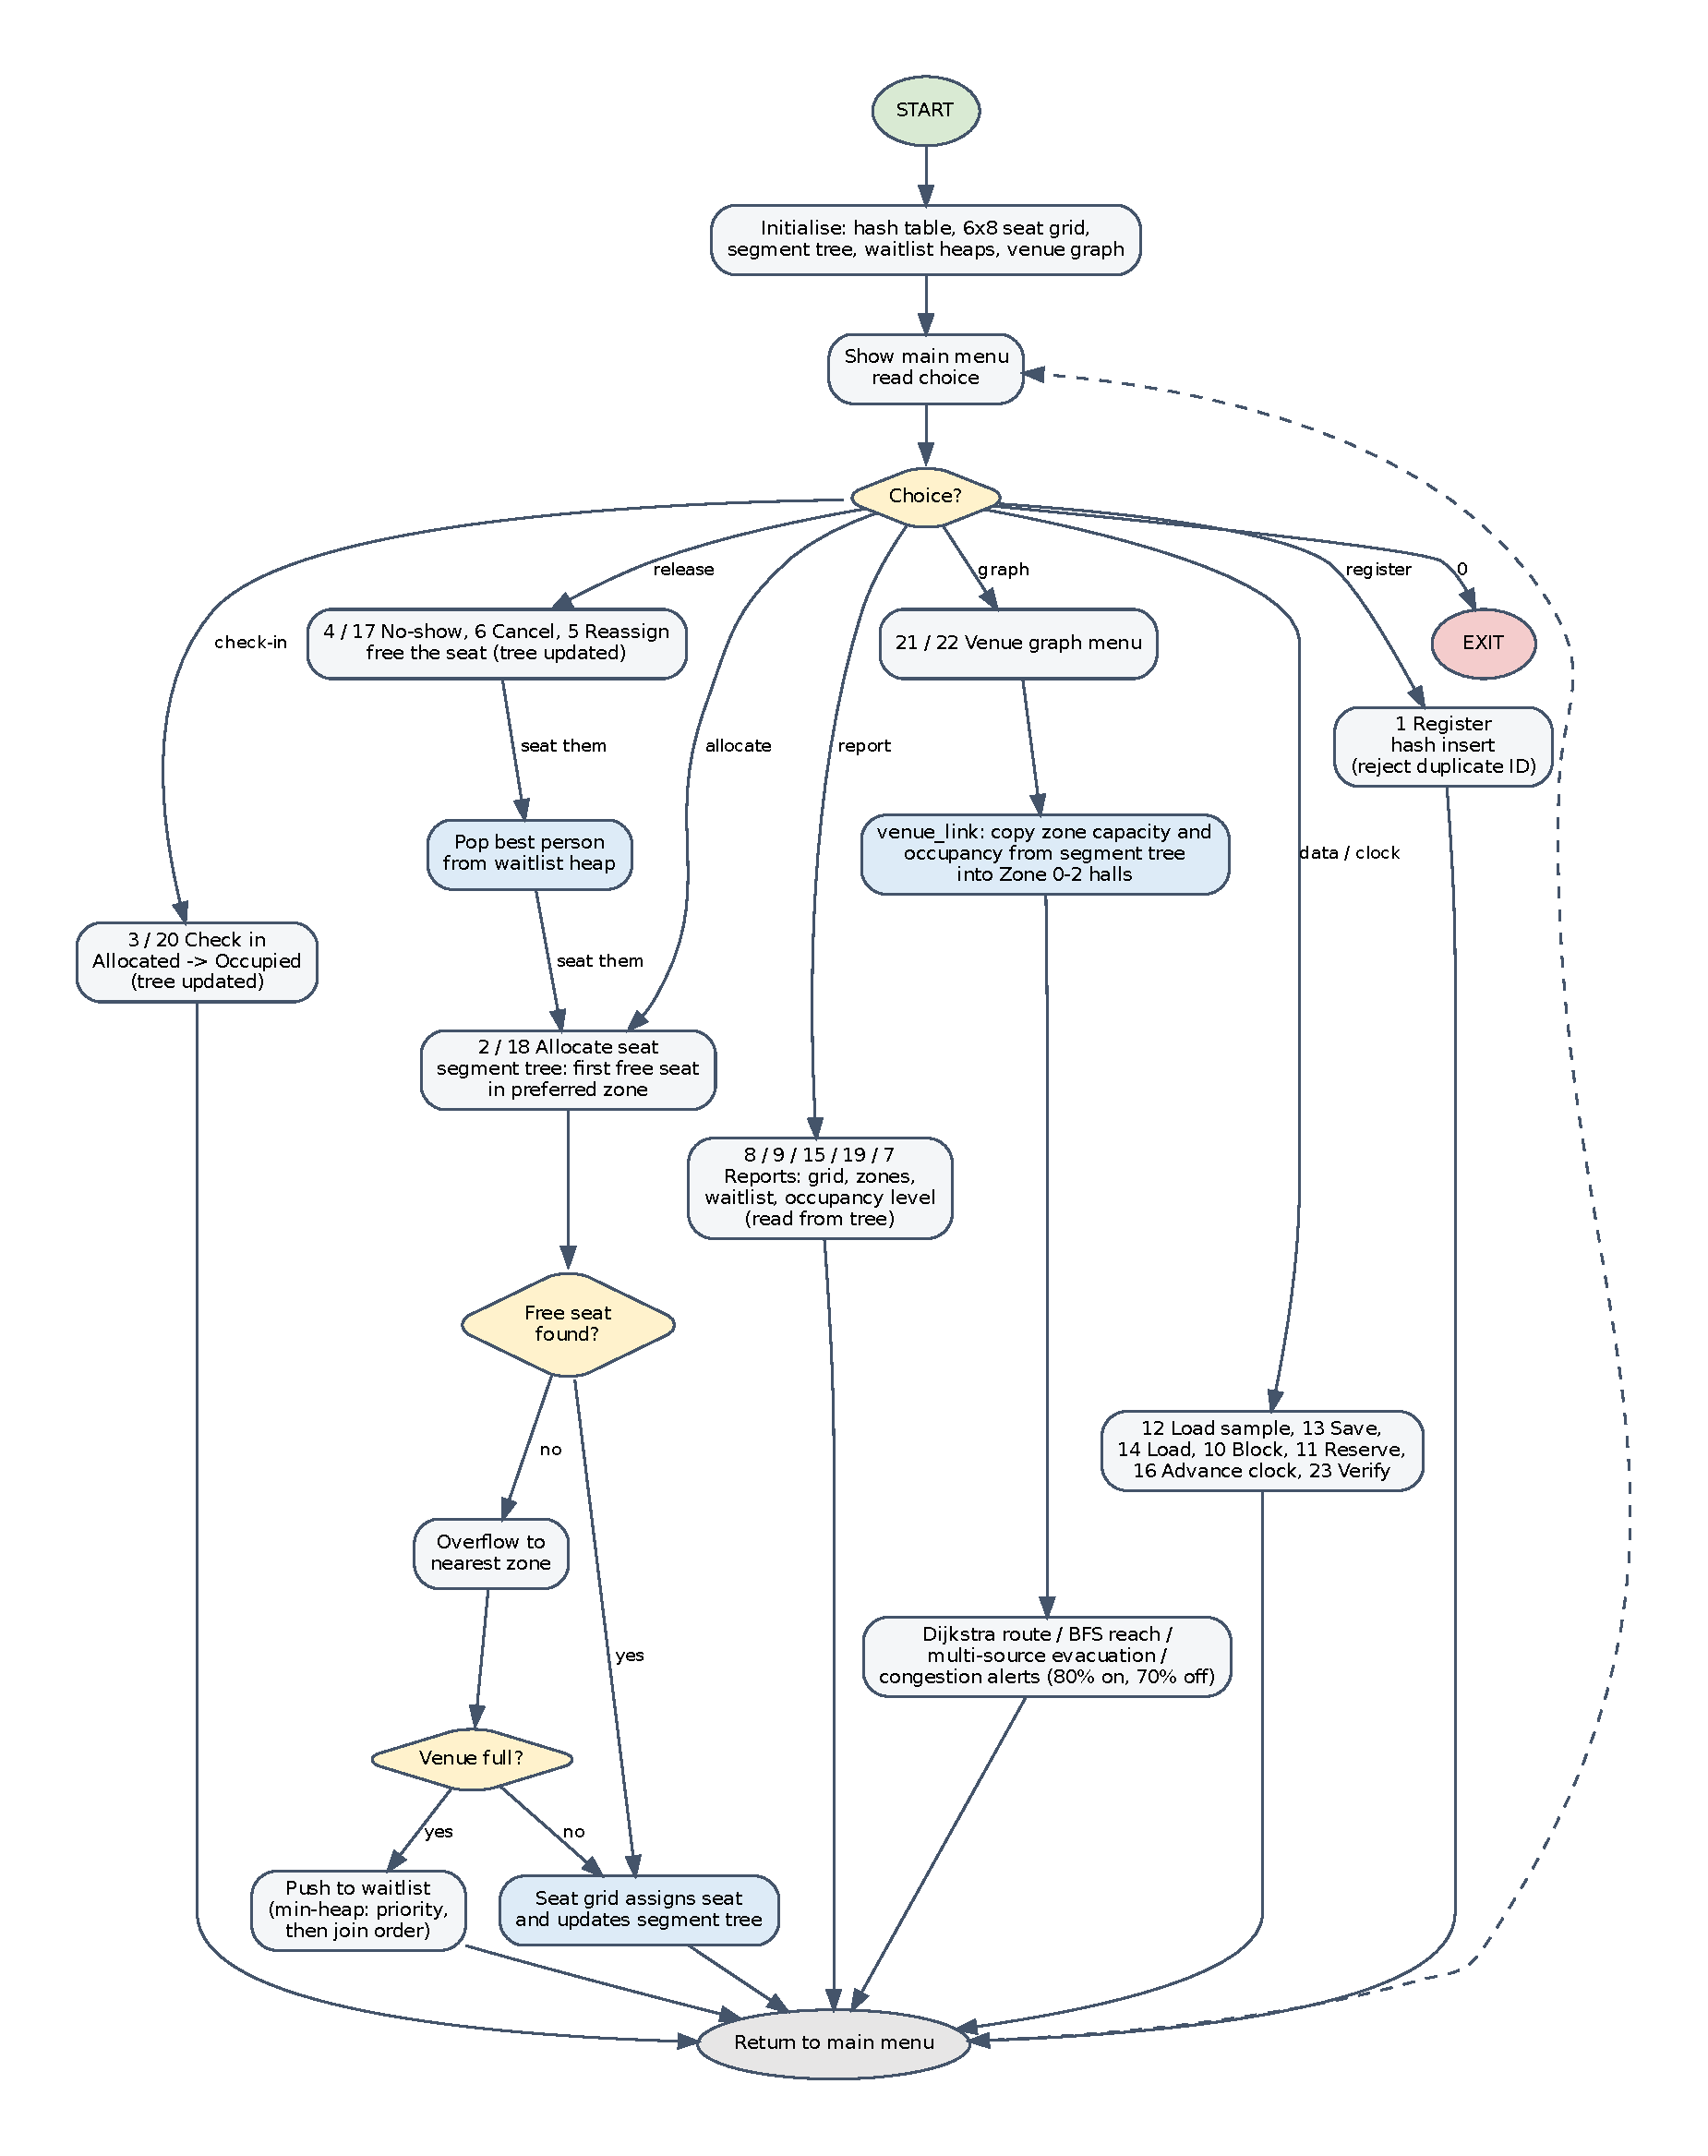
\includegraphics[height=0.62\textheight]{flowchart.pdf}
  \caption{Flow chart of CampusFlow. Shaded boxes mark steps where one data
  structure hands work to another.}
  \label{fig:flow}
\end{figure}

\subsection{Modules and how they work}

The project is divided into the modules listed in Table~\ref{tab:modules}.
For most modules, the header file contains the declarations and the source
file contains the corresponding definitions.

\begin{table}[ht]
\centering
\small
\begin{tabularx}{\textwidth}{@{}l>{\raggedright\arraybackslash}p{3.4cm}>{\raggedright\arraybackslash}X@{}}
\toprule
\textbf{Module} & \textbf{Files} & \textbf{Responsibility}\\
\midrule
Hash table & \code{hash\_table.*} & Finds a participant by ID string; chaining; doubles in size when load reaches 0.75.\\
Seat grid \& allocation & \code{seat\_grid.*}, \code{allocation.*} & Holds the state of every seat (free, allocated, occupied, blocked, reserved); allocates, reassigns, cancels; keeps the grid, hash table and tree in agreement.\\
Segment tree & \code{segment\_tree.*} & Per-range counts of free, reserved, allocated and occupied seats; point update, range query, find first free seat.\\
Waitlist & \code{waitlist\_heap.*}, \code{waitlist.*} & Min-heap per zone; no-show release and automatic promotion with the 15-minute grace period.\\
Occupancy & \code{occupancy.*} & Zone and venue report with levels LOW (below 30\%), NORMAL (below 70\%), HIGH (below 90\%), OVERCROWDED.\\
Venue graph & \code{VenueGraph.h}, \code{Config.h}, \code{graph\_menu.*} & Locations and corridors; Dijkstra, BFS, multi-source evacuation, congestion alerts with hysteresis; graph menu and custom venue setup.\\
Link & \code{venue\_link.*} & Copies zone capacity and occupancy from the segment tree into the graph.\\
Persistence & \code{persistence.*} & Saves and loads participants and blocked/reserved seats as plain text; rejects a missing, corrupt or wrong-size file without changing data.\\
Main menu & \code{main.cpp} & The 23-option menu that calls all modules.\\
\bottomrule
\end{tabularx}
\caption{Modules of CampusFlow.}
\label{tab:modules}
\end{table}

\subsubsection*{Registration and seat allocation}
When a participant registers, the system stores their details in the hash
table. It rejects the entry if the ID is empty or already exists. During seat
allocation, the segment tree is used to find the first available general seat
in the participant's preferred zone through \code{findFirstFree}. If that zone
has no free seat, the system checks the nearest zone. When every usable seat is
taken, the participant is added to the waiting list. Blocked seats are excluded
from the venue's capacity, while reserved seats are skipped during automatic
allocation.

\subsubsection*{Check-in, no-shows and the waiting list}
When a participant checks in, their seat changes from \emph{allocated} to
\emph{occupied}. Option 16 advances the simulated clock. Once 15 minutes have
passed, option 17 releases the seats belonging to participants who have not
checked in, marks those participants as NO\_SHOW and assigns the freed seats to
people from the waiting list. The heap ranks participants by higher priority
first, earlier join time second and ID as the final tie-breaker. This also makes
the selection order predictable.

\subsubsection*{Occupancy report}
To generate an occupancy report, the program queries the segment tree for
each zone and then for the venue as a whole. A participant is counted as present
only after checking in. The program uses the occupancy percentage to assign a
level, following the thresholds shown in Table~\ref{tab:modules}.

\subsubsection*{Venue graph, routing and evacuation}
The default venue map contains seven locations: \code{Gate}, \code{Junction},
\code{Zone 0}, \code{Zone 1}, \code{Zone 2}, \code{Exit East} and
\code{Exit West}. Corridors connect these locations. Each corridor is assigned
a cost using the following formula:
\[
  \text{cost} = t_{\text{normal}} \times \bigl(1 + p \times r\bigr),
\]
Here, $t_{\text{normal}}$ is the corridor's normal travel time, $p$ is its
congestion likelihood (0--1), and $r$ is the occupancy ratio at the busier end
of the corridor. Closed locations and corridors are ignored during route
calculations.

We use \emph{Dijkstra's algorithm} to find the fastest route between two
locations, and \emph{BFS} to list all locations reachable from a given point.
For evacuation, a \emph{multi-source search} starts from all open exits at the
same time. This finds the best exit for every location in one pass, while also
considering clearance times. Congestion alerts turn on when occupancy reaches
80\% of capacity and turn off when it falls to 70\%. Between these thresholds,
the alert keeps its previous state; this is the hysteresis behaviour.

\subsubsection*{Complexity summary}
\begin{table}[ht]
\centering
\small
\begin{tabularx}{\textwidth}{@{}>{\raggedright\arraybackslash}p{2.3cm}>{\raggedright\arraybackslash}p{4.4cm}>{\raggedright\arraybackslash}p{3.3cm}>{\raggedright\arraybackslash}X@{}}
\toprule
\textbf{Structure} & \textbf{Operation} & \textbf{Cost} & \textbf{Why chosen}\\
\midrule
Hash table & insert, find, erase & $O(1)$ average & Direct lookup from an ID string\\
Seat grid & change one seat & $O(1)$ & Natural 2-D layout\\
Segment tree & update, range count, first free & $O(\log N)$ & No scan of all seats\\
Min-heap & push, pop best & $O(\log W)$ & Always serves the best waiting person\\
Min-heap & cancel from the middle & $O(W)$ & Linear search by ID\\
Graph & Dijkstra / BFS & $O((V{+}E)\log V)$ / $O(V{+}E)$ & Routes with congestion cost\\
\bottomrule
\end{tabularx}
\caption{Data structures, operations and costs ($N$ seats, $W$ waiting, $V$ locations, $E$ corridors).}
\end{table}

% =================================================================
%  STEP 3 : CODING
% =================================================================
\section{Step 3: Coding}

\subsection{Modular structure}
We have kept the code organised into separate files. As required by the
assignment, declarations are placed in \code{.h} files inside \code{include/},
while definitions are placed in \code{.cpp} files inside \code{Source/}.
Compiled object files are stored in \code{object/}, and the \code{Makefile} and
executable \code{a.out} are kept in the parent directory. The complete project
contains approximately 3400 lines of code, including the tests.

\begin{lstlisting}[language={}, caption={Directory layout of the submission.}]
campusflow/
|-- Makefile, a.out
|-- include/    13 headers (.h)
|-- Source/     11 source files (.cpp), including main.cpp
|-- object/     compiled .o files
|-- tests/      5 test programs
|-- samples/    scripted inputs and expected outputs
|-- Document/   user manual
\end{lstlisting}

The project can be built and tested using the commands below. Running
\code{make} creates the \code{a.out} executable, and \code{./a.out} starts the
program. The command \code{make test} runs the test suites, while
\code{make demo} replays the sample sessions.

\subsection{Sample code}
The code samples below show how we implemented some of the main data
structures. In each case, the header file declares the interface and the source
file contains the implementation. The first example is the segment tree
interface from \code{include/segment\_tree.h}:

\begin{lstlisting}[caption={Segment tree interface (excerpt).}]
class SegmentTree {
public:
    void build(const std::vector<TreeSeat>& seats);
    void update(int idx, TreeSeat s);      // O(log N)
    Counts query(int l, int r) const;      // inclusive range, O(log N)
    int findFirstFree(int l, int r, FreeKind kind) const;   // -1 if none
private:
    int n = 0;
    std::vector<Counts> tree;              // 4*n nodes, node 1 = root
};
\end{lstlisting}

The next example is the search function from
\code{Source/segment\_tree.cpp}. It finds the first free seat in a requested
range in $O(\log N)$ time. To save work, it skips any part of the tree that has
no free seats:

\begin{lstlisting}[caption={Finding the first free seat in a range.}]
int SegmentTree::findRec(int node, int l, int r, int ql, int qr,
                         FreeKind kind) const {
    if (qr < l || r < ql) return -1;                // no overlap
    if (freeOf(tree[node], kind) == 0) return -1;   // nothing free below
    if (l == r) return l;                           // found a leaf
    int m = (l + r) / 2;
    int res = findRec(2 * node, l, m, ql, qr, kind);
    if (res != -1) return res;                      // left side wins
    return findRec(2 * node + 1, m + 1, r, ql, qr, kind);
}
\end{lstlisting}

The final example shows how the waiting-list heap compares two entries and
moves a newly inserted entry towards its correct position
(\code{Source/waitlist\_heap.cpp}):

\begin{lstlisting}[caption={Heap ordering and sift-up.}]
bool WaitlistHeap::better(const WaitEntry& a, const WaitEntry& b) {
    if (a.weight != b.weight) return a.weight > b.weight;   // priority first
    if (a.regTime != b.regTime) return a.regTime < b.regTime; // then earlier
    return a.id < b.id;                                       // then ID
}

void WaitlistHeap::siftUp(int i) {
    while (i > 0) {
        int p = (i - 1) / 2;
        if (!better(h[i], h[p])) break;
        std::swap(h[i], h[p]);
        i = p;
    }
}
\end{lstlisting}

\subsection{Honest note on standard containers}
We implemented the hash table, seat grid, segment tree, heap and graph
algorithms ourselves. However, a few parts of the program still rely on C++
standard containers. The hash table uses \code{std::list} for its buckets, and
the waiting-list module uses \code{std::unordered\_set} to track waiting IDs.
The graph module uses \code{std::unordered\_map} for name lookup,
\code{std::priority\_queue} in Dijkstra's algorithm and \code{std::queue} in BFS.
Replacing these remaining containers with our own implementations is one of
the improvements we have left for future work.

% =================================================================
%  STEP 4 : TESTING
% =================================================================
\section{Step 4: Testing}

\subsection{Automated test suites}
We used five automated test suites to check the different parts of the system.
The command \code{make test} builds and runs all five suites. A suite returns
exit code 0 only when all of its checks pass. In our final build, all five
suites completed successfully.

\begin{table}[ht]
\centering
\small
\begin{tabularx}{\textwidth}{@{}l>{\raggedright\arraybackslash}X@{}}
\toprule
\textbf{Suite} & \textbf{What it covers}\\
\midrule
\code{test\_all} & Hash table (collisions, resize, duplicates), seat grid, allocation, zone overflow, tree/grid agreement, save/load, edge cases.\\
\code{test\_waitlist} & Priority and zone order, no-show release, empty waiting list, a randomised run with 1604 people.\\
\code{test\_occupancy} & Level thresholds, per-zone levels, edge cases, last-seat case, comparison with a brute-force count.\\
\code{test\_graph} (117 checks) & Graph validation, Dijkstra (disconnected, closed location, closed corridor, congestion changing the route), BFS, multi-source evacuation (several exits, closed exit, all exits closed), hysteresis, capacity update.\\
\code{test\_integration} (178 checks) & Whole system: registration to check-in feeding the graph; alerts driven by cancellations; waiting list and no-show flow; evacuation reroute; save/load round trip; 3000-step random stress test comparing the segment tree with brute-force counts.\\
\bottomrule
\end{tabularx}
\caption{Automated test suites.}
\end{table}

\subsection{Test data}
\begin{itemize}
  \item Venue: $6\times 8$ grid, 48 seats, 3 zones of 16 seats; no-show grace period 15 minutes.
  \item Option 12 registers participants \code{P101, P102, \dots} with rotating priority 0--2 and rotating preferred zone; the demo uses 50, plus one hand-entered participant \code{A100} (priority 5, zone 1), so 51 people in total.
  \item Seat (5,7) is blocked and seat (5,6) is reserved, leaving 46 usable seats.
  \item Three scripted sessions in \code{samples/}: \code{full\_demo}, \code{custom\_venue} and \code{edge\_cases}.
\end{itemize}

\subsection{Functional test cases}
The test cases in Table~\ref{tab:cases} are taken from the scripted
\code{full\_demo} session. When we run \code{make demo}, the program replays the
session and checks its output against the saved expected output. All three
sample sessions match their expected results. We also checked that the program
exits cleanly if the input ends before the user completes an operation.

{\small
\begin{longtable}{@{}>{\raggedright\arraybackslash}p{0.7cm}>{\raggedright\arraybackslash}p{3.2cm}>{\raggedright\arraybackslash}p{3.6cm}>{\raggedright\arraybackslash}p{7.2cm}@{}}
\caption{Functional test cases (from \code{samples/full\_demo\_input.txt}).}\label{tab:cases}\\
\toprule
\textbf{No.} & \textbf{Function} & \textbf{Input} & \textbf{Expected result (observed: pass)}\\
\midrule
\endfirsthead
\toprule
\textbf{No.} & \textbf{Function} & \textbf{Input} & \textbf{Expected result (observed: pass)}\\
\midrule
\endhead
\bottomrule
\endlastfoot
1 & Register & Option 1, \code{A100} & Participant registered\\
2 & Duplicate ID & Option 1, \code{A100} again & Rejected: ID already exists\\
3 & Unknown participant & Option 7, \code{NOPE} & Reports not found\\
4 & Load sample data & Option 12, 50 & 50 participants \code{P101}--\code{P150}\\
5 & Block / reserve seat & Option 10 (5,7); option 11 (5,6) & Seat blocked; seat reserved; 46 seats usable\\
6 & Full venue & Option 18 & 46 seated, 5 waitlisted\\
7 & Waiting list order & Option 15 & Per zone, higher priority first, then earlier join\\
8 & Consistency & Option 23 & ``Consistent: hash table, seat grid and segment tree agree''\\
9 & Check-in a zone & Option 20, zone 0 & 16 checked in; Zone 0 is 100.0\% and OVERCROWDED\\
10 & Evacuation & Option 21, then 8, \code{Zone 0} & Route Zone 0 $\to$ Exit West, cost 46.00 s\\
11 & Fastest route & Graph option 6, \code{Gate} to \code{Exit East} & Gate $\to$ Junction $\to$ Zone 2 $\to$ Exit East, 52.00 s\\
12 & Closed exit reroute & Close \code{Exit West}, then option 8, \code{Zone 0} & Route changes to Zone 0 $\to$ Zone 1 $\to$ Zone 2 $\to$ Exit East, 96.00 s\\
13 & Early no-show check & Advance clock 10, then option 17 & Refused: grace period not over\\
14 & No-show release & Advance clock 5 more, then option 17 & 14 no-show seats released; 5 waiting people seated in priority order\\
15 & Reassign seat & Option 5, \code{P148} to (4,0) & Reassigned; grid shows the move\\
16 & Cancel & Option 6, \code{P101} & Cancelled; participant shows CANCELLED\\
17 & Save and load & Options 13 and 14 & State restored; still consistent\\
\end{longtable}
}

\subsection{Edge cases}
The \code{edge\_cases} session covers situations that could cause problems in
normal use. These include invalid numbers, unknown IDs, duplicate registrations,
invalid seat positions, checking for no-shows too early, files that are missing
or cannot be written, all exits being closed, and crowd values outside the
allowed range. If a save file is missing, corrupt or has the wrong size, the
program rejects it without changing the current data.

\subsection{A defect found by testing}
We found one defect while combining the work from all three team members.
When a seat was reassigned to someone who had already checked in, the
participant's record still showed them as checked in, but the new seat was
marked only as \emph{allocated}. As a result, the occupancy report did not count
that participant as present. We fixed the issue with a one-line change in
\code{allocation.cpp} and added an integration test so that the same problem is
caught if it appears again.

% =================================================================
%  STEP 5 : CONTRIBUTIONS, TAKEAWAYS, ETC.
% =================================================================
\section{Step 5: Contributions, Key Takeaways and References}

\subsection{Individual contributions}
The work was divided across the three team members so that each person could
focus on a set of related modules. Table~\ref{tab:files} records the files
handled by each member and summarises their main contributions.

\begin{table}[H]
\centering
\small
\begin{tabularx}{\textwidth}{@{}>{\raggedright\arraybackslash}p{3.3cm}>{\raggedright\arraybackslash}p{5.2cm}>{\raggedright\arraybackslash}X@{}}
\toprule
\textbf{Member} & \textbf{Files owned} & \textbf{Main contribution}\\
\midrule
\MemberOne\ (\RegOne) & \code{common.h}, \code{hash\_table.*}, \code{seat\_grid.*}, \code{allocation.*}, \code{persistence.*}, \code{test\_all.cpp} & Hash table, seat grid, seat allocation, zone overflow, reassign and cancel, save/load, and their tests.\\
\MemberTwo\ (\RegTwo) & \code{segment\_tree.*}, \code{waitlist\_heap.*}, \code{waitlist.*}, \code{occupancy.*}, \code{test\_waitlist.cpp}, \code{test\_occupancy.cpp} & Segment tree, waiting-list heap, check-in and no-show handling, occupancy report, and their tests.\\
\MemberThree\ (\RegThree) & \code{Config.h}, \code{VenueGraph.h}, \code{graph\_menu.*}, \code{test\_graph.cpp} & Venue graph, Dijkstra, BFS, evacuation, congestion alerts, analytics, crowd simulation, graph menu, and tests.\\
\textit{Shared} & \code{main.cpp}, \code{venue\_link.*}, \code{test\_integration.cpp}, \code{Makefile}, \code{samples/} & Main menu, link from the tree to the graph, integration tests, build file and sample sessions.\\
\bottomrule
\end{tabularx}
\caption{Files owned by each member.}
\label{tab:files}
\end{table}

\subsection{Key takeaways}
\begin{itemize}
  \item We learned how useful a \textbf{segment tree} can be for handling both zone-wise counts and first-free-seat queries in $O(\log N)$. Using it as the common source of occupancy data also helped us avoid inconsistent counts.
  \item A \textbf{min-heap} can do more than store values by size. By comparing priority, join time and ID, we were able to make waiting-list selection fair and predictable.
  \item The \textbf{hash table} and its resizing logic helped us keep participant lookup close to $O(1)$ on average as the number of registrations increased.
  \item Using \textbf{Dijkstra, BFS and multi-source search} on the same venue graph showed us how different graph algorithms can solve different movement-related problems. Including congestion in the edge cost can also change the route that is selected.
  \item Working with a \textbf{modular codebase}, a Makefile and separate tests made it easier for three people to develop different parts in parallel. The integration tests were especially useful because they exposed a defect that had not been caught earlier.
\end{itemize}

\subsection{Future scope}
\begin{itemize}
  \item Include the waiting list in saved data. At present, it has to be rebuilt using option 18 after a file is loaded.
  \item Replace the standard containers that are still used in a few modules with our own implementations.
  \item Develop a graphical or web-based interface and support live head-counts through QR or RFID check-in.
  \item Add an option to switch from a custom venue graph back to the default graph without restarting the program.
\end{itemize}

\subsection{Acknowledgements}
We are grateful to our course instructor for providing the project problem
statement and guiding us throughout CSLR31. We also thank the laboratory staff
for their support and acknowledge the effort and cooperation of all our team
members in completing the project.

\begin{thebibliography}{9}
\bibitem{unesco-sdg} UNESCO, \emph{Sustainable Development Goals}. \url{https://www.unesco.org/en/sdgs}
\bibitem{clrs} T.~H.~Cormen, C.~E.~Leiserson, R.~L.~Rivest and C.~Stein, \emph{Introduction to Algorithms}, MIT Press (heap, hash table, graph search and Dijkstra's algorithm).
\bibitem{dijkstra} E.~W.~Dijkstra, ``A note on two problems in connexion with graphs'', \emph{Numerische Mathematik}, 1:269--271, 1959.
\bibitem{cppref} cppreference.com, \emph{C++ reference} (standard library containers used).
\bibitem{make} GNU Make Manual, \url{https://www.gnu.org/software/make/manual/}
\end{thebibliography}


\end{document}